\begin{frame}[t]{Die Messbruecke - realer PTC KTY81-210} 
    
    \begin{spacing}{0.9} \begin{tiny}
      \begin{table}[h!]
      \begin{tabular}{p{10cm}}
        \hline
        \textbf{Das Bauteil KTY81-210} \\
        \hline \\
        \begin{minipage}{\textwidth}
            Der KTY81-210 ist ein PTC und wir wollen ihn als Temperaturfühler in unserer Brückenschaltung verwenden.\newline
            Dazu müssen wir ihn in LTspice modellieren.\newline\newline Um das entsprechende Verhalten nachzubilden benötigen wir die 
            Spezifikation des Sensors aus seinem Datenblatt.
            \begin{itemize}
                \item Ihr könnt das Hersteller-Datenblatt hier \href{https://cdn-reichelt.de/documents/datenblatt/B400/KTY81-2\%23PHI.pdf}{ $ << Hyperlink\ zum\ PDF >> $} herunterladen
                \item Ihr könnt die Hersteller-Formelreferenz hier \href{https://www.mikrocontroller.net/attachment/243481/KTY-Philips.pdf}{$ << Hyperlink\ zum\ PDF >> $} herunterladen
            \end{itemize}
            

        \end{minipage} 
        \\ \\
        \hline
        \textbf{Analyse des Datenblattes} \\
        \hline \\
        \begin{minipage}{\textwidth}
            Das Datenblatt enthält eine Tabelle die die Widerstandswerte über die Temparatur beschreibt. \newline

            \begin{tabular}{p{3cm} p{8cm}}
                \begin{minipage}{.3\textwidth}
                    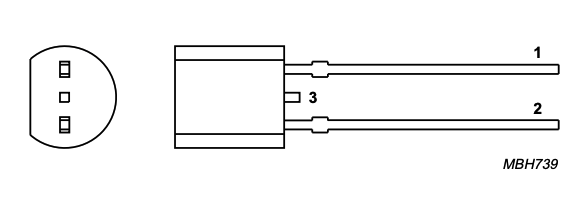
\includegraphics[width=0.8\linewidth]{pictures/kty81_overview.png}
                    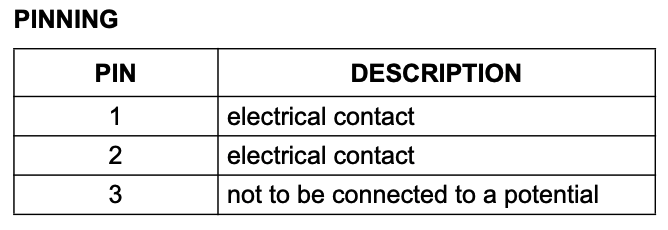
\includegraphics[width=0.8\linewidth]{pictures/kty81_pinning.png}
                    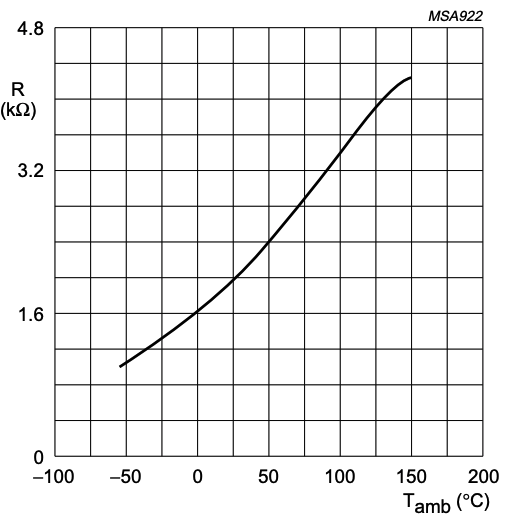
\includegraphics[width=0.8\linewidth]{pictures/kty81_graph.png} 
                \end{minipage}
            & 
                \begin{minipage}{.7\textwidth}
                    \begin{figure}
                        \centering
                        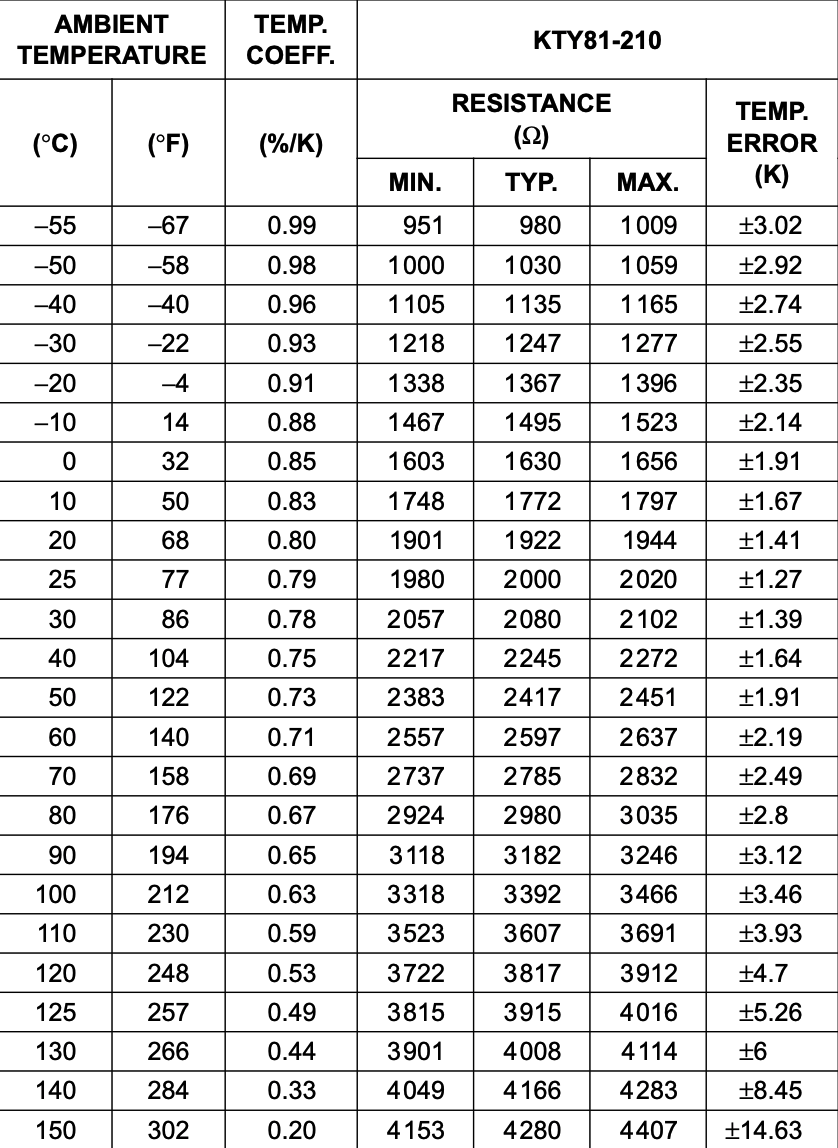
\includegraphics[width=0.45\linewidth]{pictures/kty81_table.png} 
                    \end{figure}
                \end{minipage}
            \end{tabular}
        \end{minipage} 
        \\
      \end{tabular}

    \end{table}
     
    \end{tiny} \end{spacing}

\end{frame}

\begin{frame}[t]{Die Messbruecke - Approximation eines PTC} 
    
    \begin{spacing}{0.9} \begin{tiny}
      \begin{table}[h!]
      \begin{tabular}{p{10cm}}
        \hline
        \textbf{Quadratische Approximationsformel} \\
        \hline \\
        \begin{minipage}{\textwidth}
            Der Hersteller gibt in seinem Datenblatt eine Approximationsformel zur Modellierung des Verhaltens an.

            \begin{equation}
                R_T=R_{Ref}[1+A(T-T_{Ref})+B(T-T_{Ref})^2+C(T-T_{i}^D)]
            \end{equation}
            \begin{figure}
                \centering
                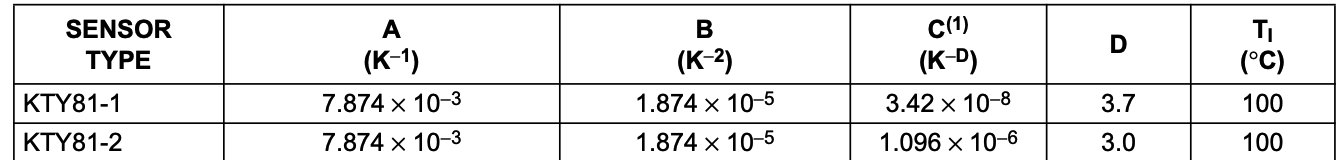
\includegraphics[width=0.6\textwidth]{pictures/kty81_constants.png}
                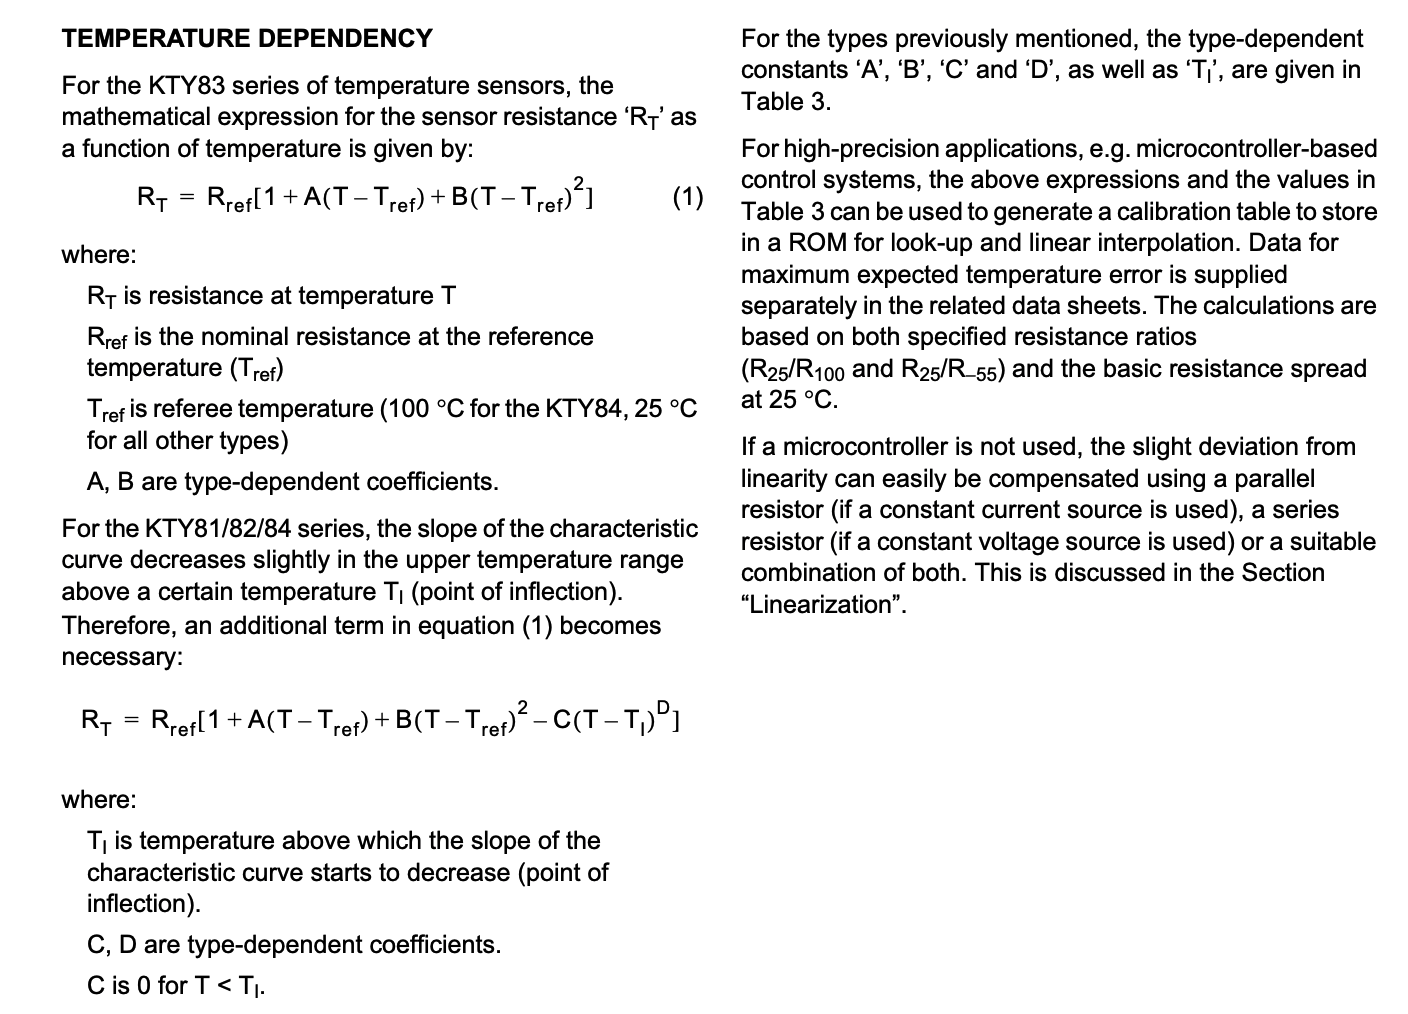
\includegraphics[width=0.6\textwidth]{pictures/kty81_formula.png}
            \end{figure}
        \end{minipage} 
    \end{tabular}

    \end{table}
     
    \end{tiny} \end{spacing}

\end{frame}

\begin{frame}[t]{Die Messbruecke - Approximation eines PTC} 
    
    \begin{spacing}{0.9} \begin{tiny}
      \begin{table}[h!]
      \begin{tabular}{p{10cm}}
        \hline
        \textbf{Genauigkeit Approximation} \\
        \hline \\
        \begin{minipage}{\textwidth}
            Wenn wir die Tabelle aus dem Datenblatt mit der quadratischen Approximationsformel (Formel 6, $C=0$) vergleichen ergibt sich folgender Verlauf.
            \begin{figure}
                \centering
                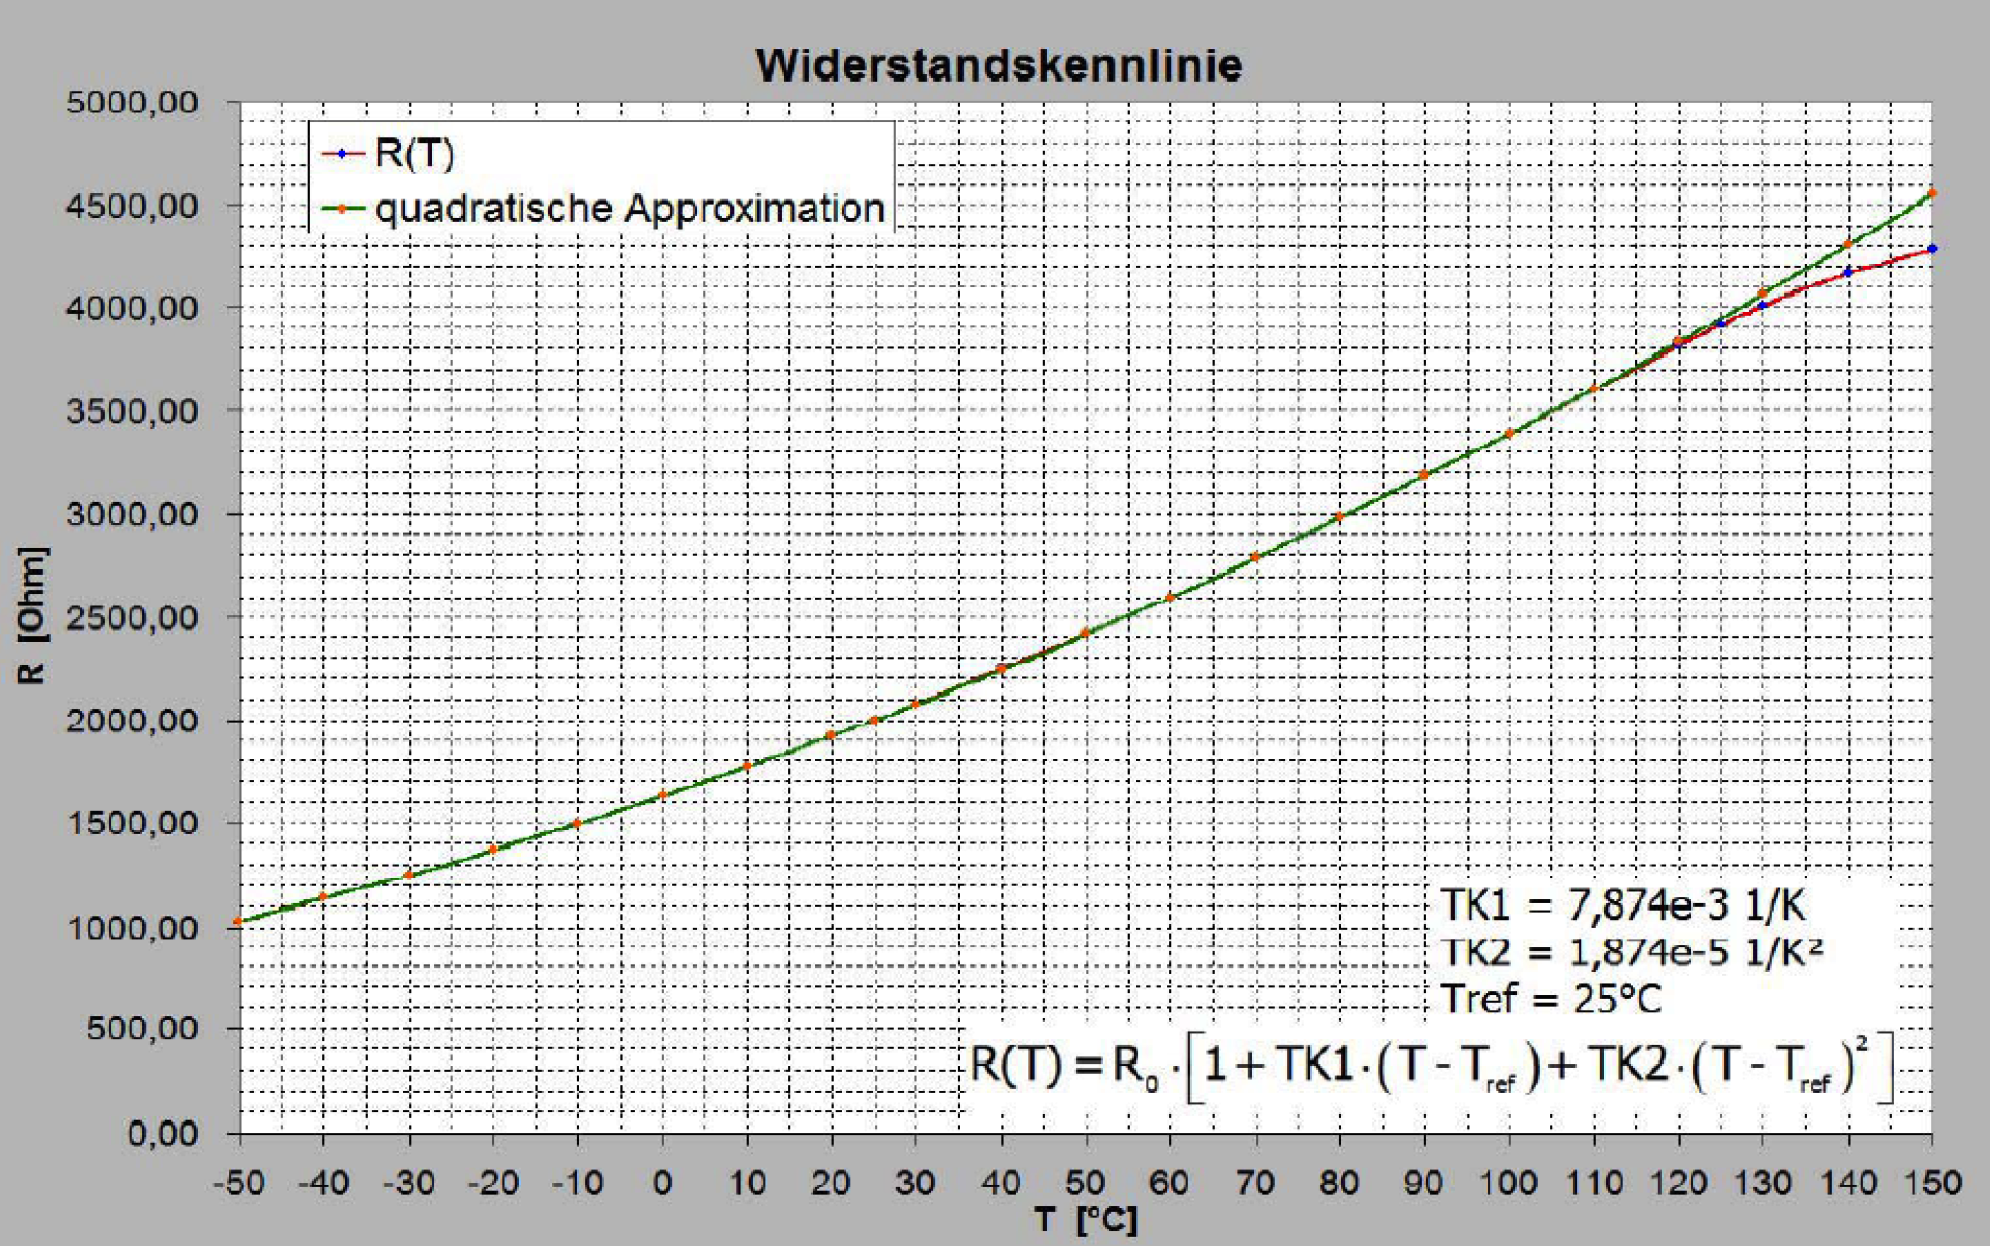
\includegraphics[width=0.6\textwidth]{pictures/kty81_approx_accuracy.png}
            \end{figure}
            Aus Formel 6 wissen wir, dass die quadratische Approximation ab einer Temparatur $T>T_i$ nicht mehr vollständig ist. 
            Diesen Effekt sehen wir hier. Ab $T>T_i=100$ weicht der reale Verlauf ab. Wenn wir unseren Messbereich jedoch auf -50$°$C - 100$°$C begrenzen, können
            wir die quadratische Formel verwenden. \newline\newline Dies werden wir im nächsten Schritt tun. 
        \end{minipage} 
    \end{tabular}

    \end{table}
     
    \end{tiny} \end{spacing}

\end{frame}

\begin{frame}[t]{Die Messbruecke - Modellierung des KTY81-210} 
    
    \begin{spacing}{0.9} \begin{tiny}
      \begin{table}[h!]
        \begin{tabular}{p{10cm}}
            \hline
            \textbf{Widerstandsformel als Variable} \\
            \hline \\
            \begin{minipage}{\textwidth}
                Zur Modellierung starten wir mit einem einfachen schematic.
            \end{minipage}
            \\ \\
        \end{tabular}
        \begin{tabular}{p{3cm} p{7cm}}
            \begin{minipage}{.3\textwidth}
                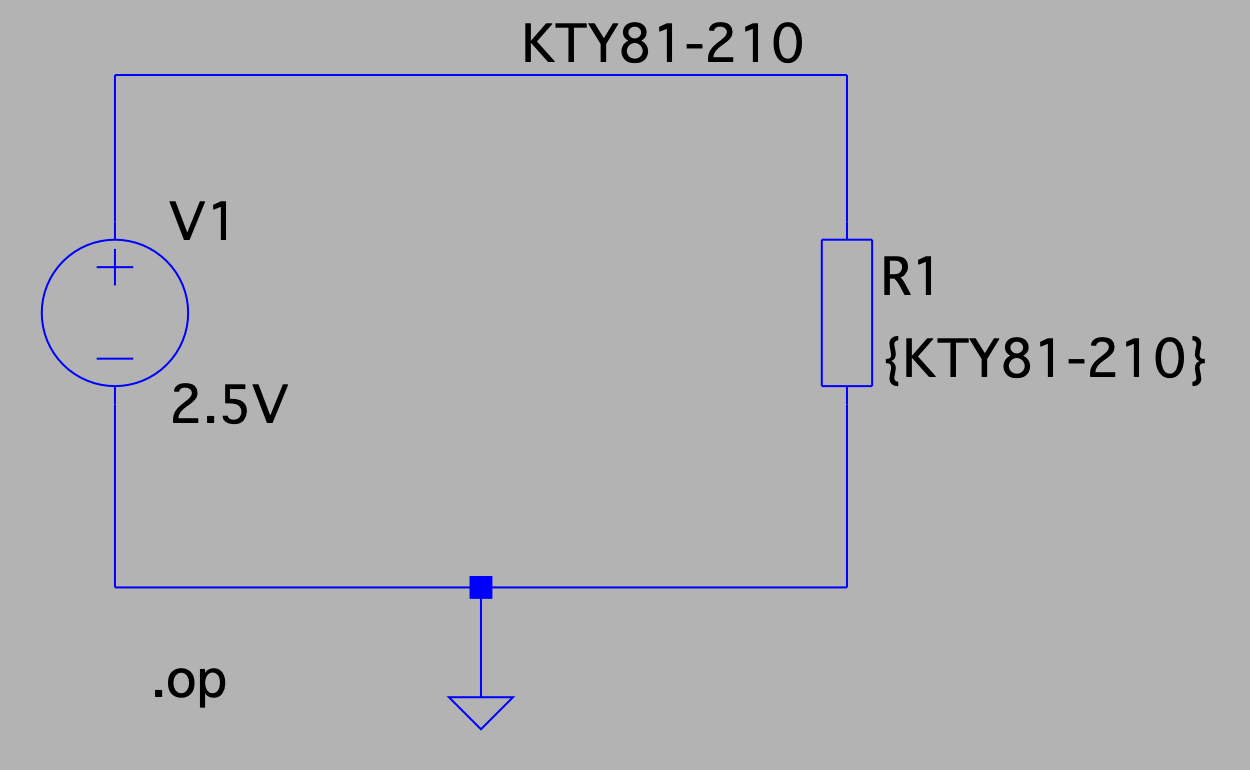
\includegraphics[width=0.8\linewidth]{pictures/kty81_test.png} 
            \end{minipage} 
            &
            \begin{minipage}{.7\textwidth}
                \begin{itemize}
                    \item Baut den Schaltplan auf
                    \item Gebt dem Widerstand $R_1$ eine Variable $KTY81-210$ als Wert
                    \item Erstellt ein Label mit dem Namen $KTY81-210$ 
                \end{itemize}
            \end{minipage} 
            \\\\
        \end{tabular}
        \begin{tabular}{p{10cm}}
            \begin{minipage}{\textwidth}
                Um den Widerstand abhängig von der Temparatur und seiner Formel zu simulieren gehen wir wie folgt vor:
                \begin{itemize}
                    \item Schrittweite Steigerung der Temparatur
                    \item Simulation entsprechend Formel 6 mit $R_{Ref}=2k$ $A=7.874^{-3}$ $B=1.874^{-5}$ $T_{Ref}=25$
                    \item $R_{KTY81-210}=2k[1+7.874^{-3}(T-25)+1.874^{-5}(T-25)^2]$
                \end{itemize}
            \end{minipage}
            \\ \\
        \end{tabular}
        \begin{tabular}{p{3cm} p{7cm}}
            \begin{minipage}{.3\textwidth}
                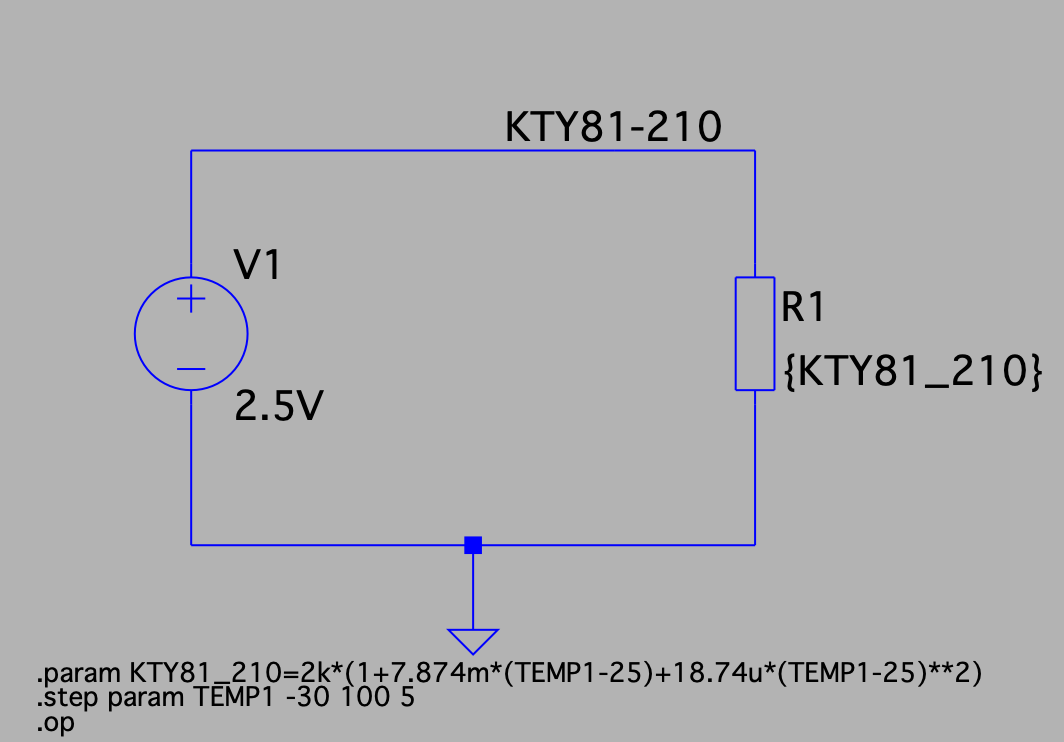
\includegraphics[width=0.8\linewidth]{pictures/kty81_simulation.png} 
            \end{minipage} 
            &
            \begin{minipage}{.7\textwidth}
                \begin{itemize}
                    \item Ihr könnt für die Variable eine Formel über die Spice-Direktive $.param$ hinterlegen
                    \item Über die Spice-Direktive $.step$ könnt ihr einen Parameter $TEMP1$ (nicht $TEMP$ dieser beschreibt die globale Temparatur) für die Tempartur einführen und variieren.
                    \item In einer Arbeitspunktanalyse können wir uns nun den trace von $R_1=\frac{V(KTY81-210)}{I(R_1)}$ anzeigen lassen. 
                \end{itemize}
            \end{minipage} 
            \\\\\\
        \end{tabular}
        \begin{tabular}{p{10cm}}
            \begin{minipage}{\textwidth}
                \begin{center}   
                    \textbf{Entspricht der Verlauf dem des Datenblattes und euren Erwartungen? \newline
                            Wenn ja, dann können wir diesen Widerstand nun in unsere Messbruecke übernehmen.}
                \end{center}
            \end{minipage}
            \\ \\
        \end{tabular}
      \end{table}
    \end{tiny} \end{spacing}

\end{frame}